Fritz ist am 4. März 1893 geboren. Seine schriftlichen Lebenserinnerungen umfassen den Zeitraum von seinen ersten Erinnerungen bis zum Anfang der 1950er Jahre. Über den weiteren Zeitraum bis zu seinem Tod am 25. Mai 1981, d.h. über die Zunahme der Repressalien in der DDR, über den Volksaufstand und dessen Niederschlagung von den Russen im Juni 1953, den Umzug Ende 1953 nach Potsdam, die Flucht in den Westen im Januar 1956, den \enquote{2. Neustart} in Berlin und den Mauerbau im August 1961 gibt es leider keine Aufzeichnungen von ihm. Wann Fritz mit den Aufzeichnungen begann, und wann er sie beendete, ist nicht bekannt. Die letzte Datierung ist vom 17.2.77, als er nach einem (zum Glück misslungenen) Überfall einen Herzinfarkt erlitten hatte und sich in einem Sanatorium in Bad Lauterberg erholte.

\begin{figure}[p]
	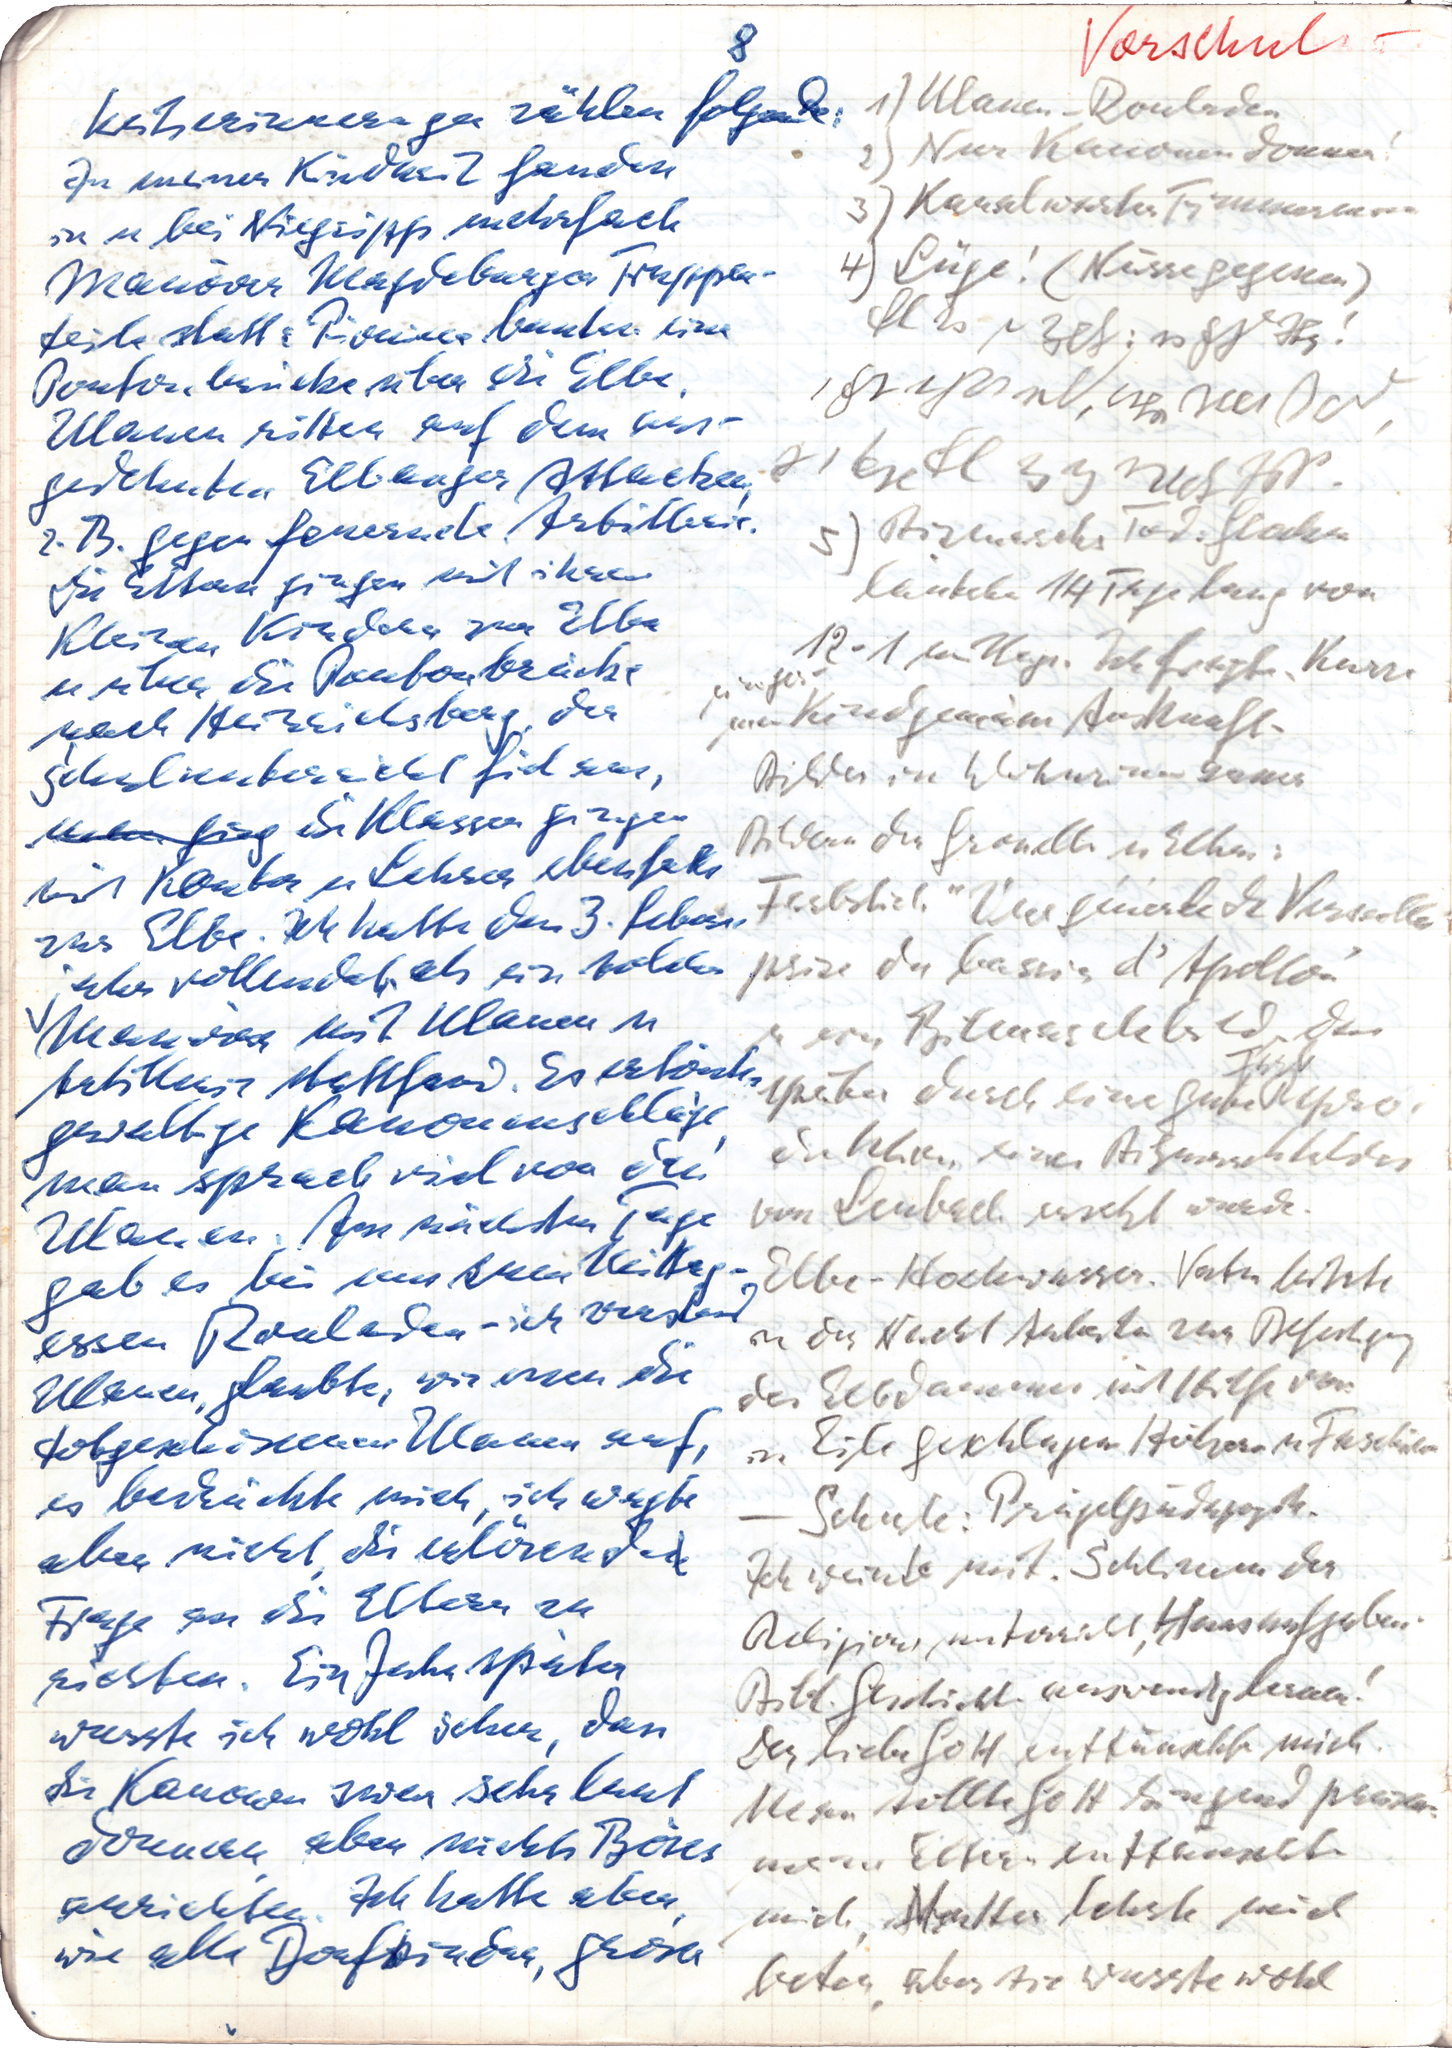
\includegraphics[width=\linewidth]{Photos/Doppelseite-links.png}
	\caption{Beispielseite, links}
	\label{fig:doppelseite_links}
\end{figure}

\begin{figure}[p]
	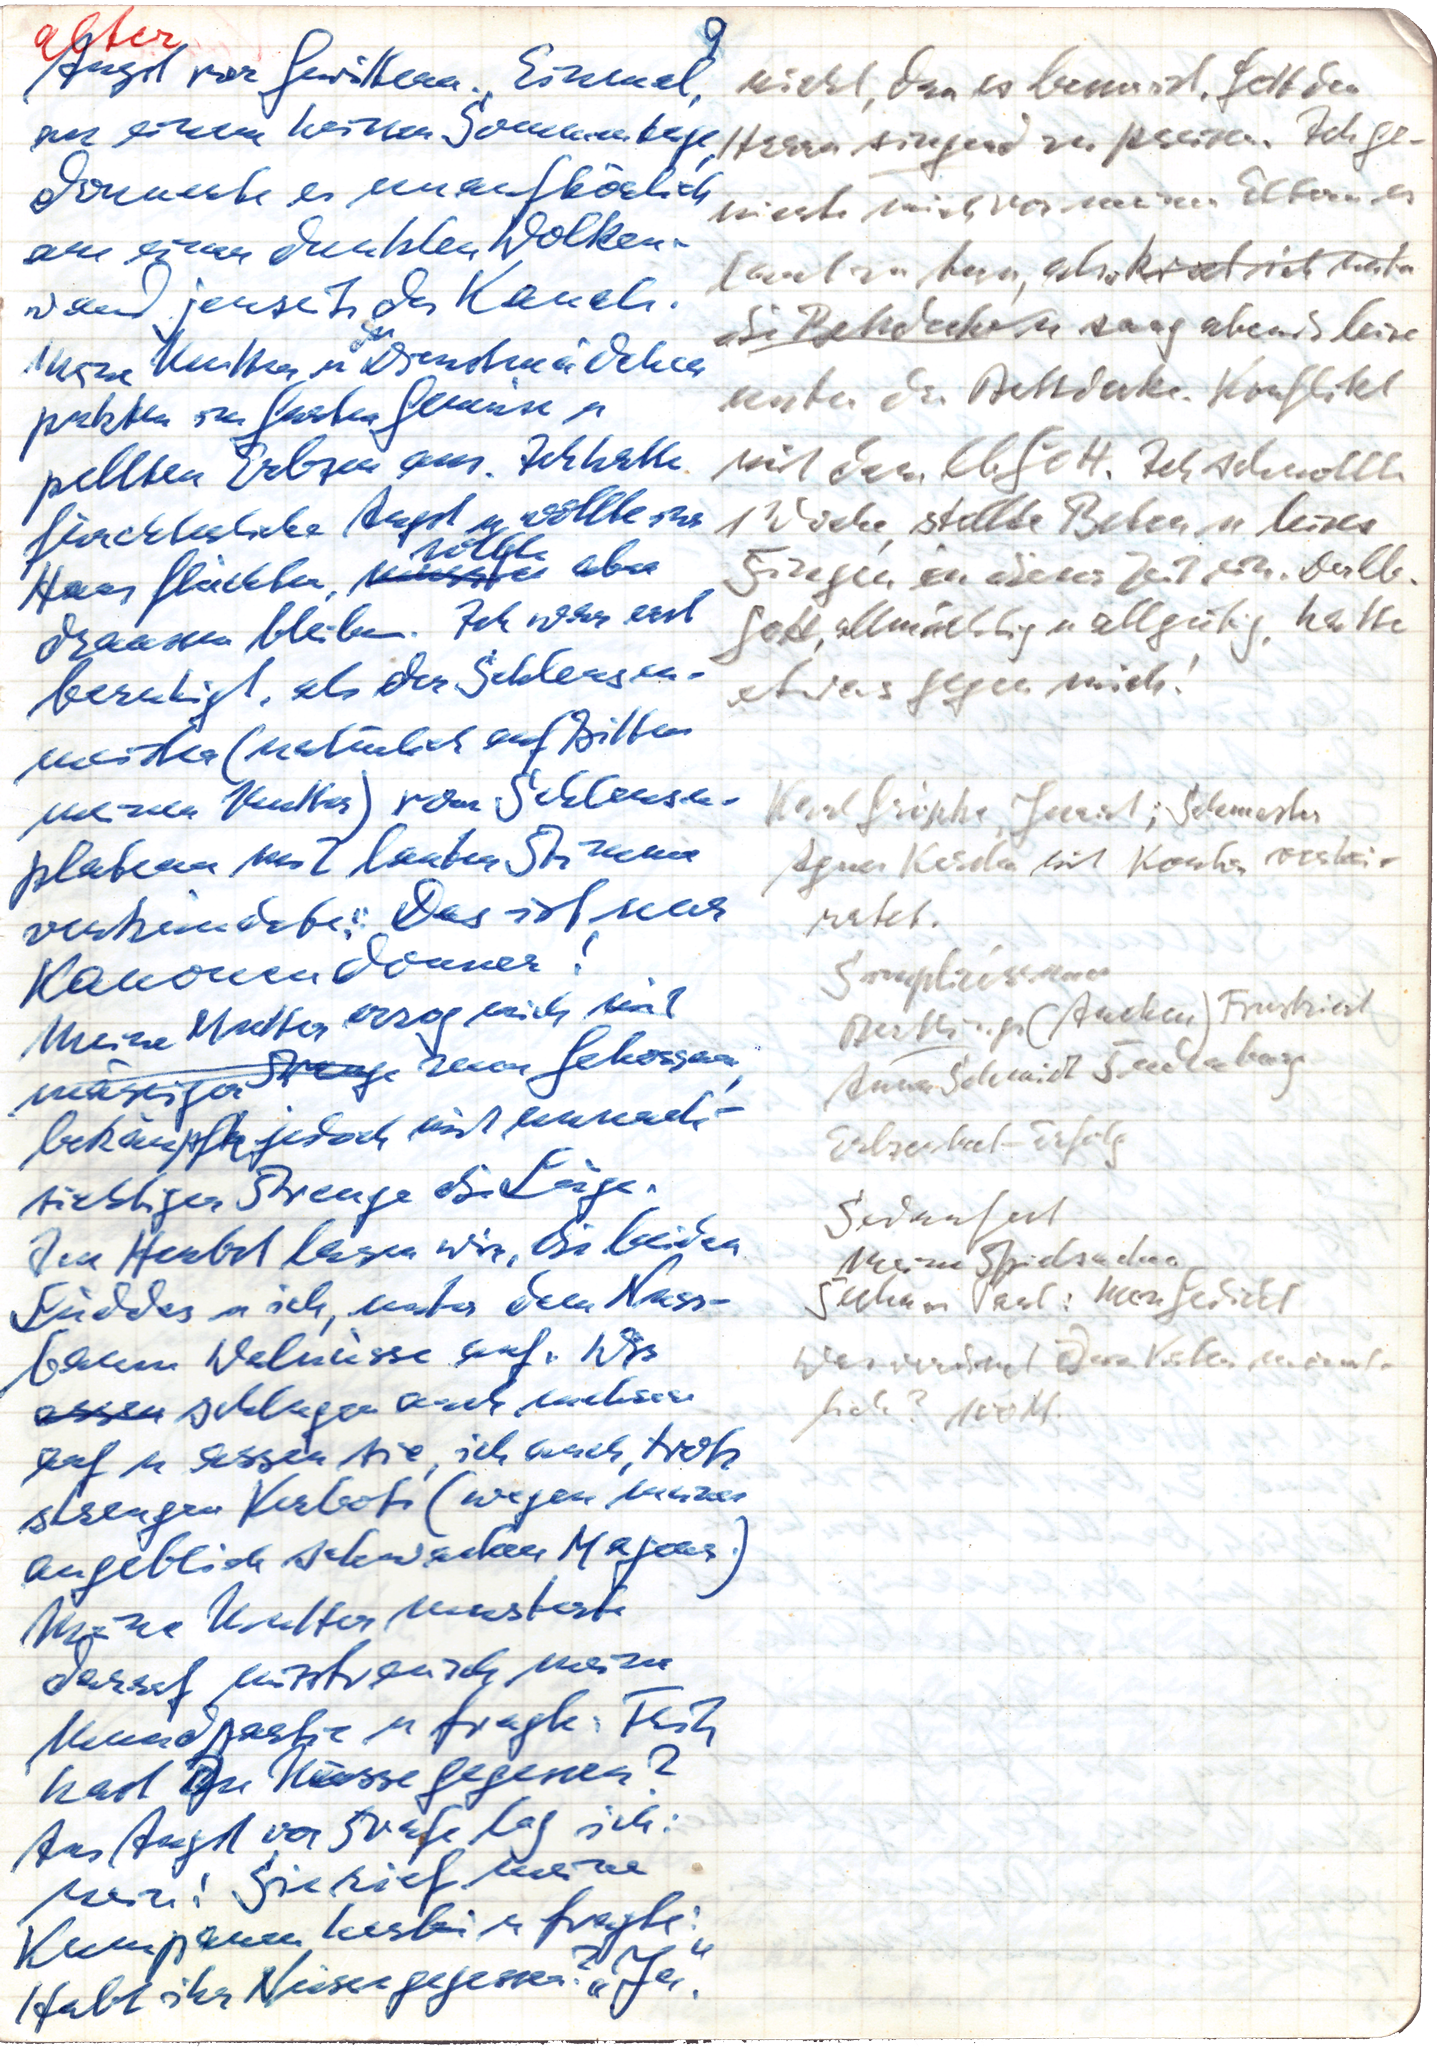
\includegraphics[width=\linewidth]{Photos/Doppelseite-rechts.png}
	\caption{Beispielseite, rechts}
	\label{fig:doppelseite_rechts}
\end{figure}

Nach Erinnerung von Helga hat Fritz seine Ideen und Formulierungen häufig Margot vorgetragen, die dann ihrerseits Anregungen gab und Anmerkungen machte. Dies fand zum großen Teil auch während der Aufenthalte in Barnave statt, wo Fritz und Margot häufig den Sommer verbrachten (manchmal schon ab Mai und bis in den September!).\\

Die Aufzeichnungen von Fritz befinden sich in 7 DIN-A5-Oktavheften mit dem Titel \enquote{Meine Lebenserinnerungen im Abriss} auf insgesamt 707 Seiten. Mit blauem Kugelschreiber hat Fritz in sehr enger und kleiner Schrift chronologisch geordnet seine Lebenserinnerungen aufgezeichnet. Vermutlich hat er in mehreren Heften gleichzeitig geschrieben: das Oktavheft, das mit seiner Kindheit beginnt, ähnelt äußerlich dem Oktavheft, das die Ereignisse ab März 1945 beschreibt, auch beginnt er in beiden Heften mit der Seitenzahl \enquote{1}. Die Seitenzahlen in den übrigen Heften führen die Nummerierung des jeweils vorigen Heftes fort.

Für die Aufzeichnungen hat Fritz die Seiten immer in der Hälfte gefaltet und zunächst nur den linken Teil beschrieben. Der rechte Teil war freigelassen für Verbesserungen und Ergänzungen, die ihm später eingefallen sind. Im ersten Oktavheft hat er zu Beginn mit rotem Kugelschreiber den Doppelseiten eine \enquote{Überschrift} gegeben. Da dies jedoch keine 10 Seiten durchgehalten wurde, hat Konstantin eine eigene Gliederung für die Aufzeichnungen erstellt. In den letzten beiden Heften von Fritz ist seine Schrift deutlich kleiner als in den vorherigen Heften, deswegen war zum Entziffern häufig eine Lupe notwendig. Vereinzelt enthalten die Hefte Notizen aus seinem Alltag (z.B. Personen- oder Buchnamen sowie zu klärende Fragen), oft schwer lesbar oder sogar in Stenographie. Sie werden hier nicht wiedergegeben, da sie offenkundig keine relevanten Informationen enthalten. Die Abbildungen \ref{fig:doppelseite_links} und \ref{fig:doppelseite_rechts} vermitteln einen Eindruck der Oktavhefte (Transskription siehe S. \pageref{para:kindheitserinnerungen}).\\

Die Tagebücher wurden von Helga handschriftlich in 3 große DIN-A4-Hefte übertragen. Orts- und Eigennamen wurden soweit möglich plausibilisiert und ggf. korrigiert. Fritz hat grundsätzlich kein \enquote{ß} benutzt, sondern immer \enquote{ss} geschrieben. Dies wurde an die aktuelle Rechtschreibung angepasst, um die Leserlichkeit zu verbessern. Ergänzungen sowie bei kyrillischen Wörtern die Transliteration sind in eckigen Klammern gesetzt, Erläuterungen oder Erinnerungen von Helga wurden als Fußnoten eingefügt.

Den Großteil der Abschrift machte Helga von Juli 1997 bis 2002 während der Sommerferien in Barnave, den Teil ab März 1945 (d.h. Kapitulation, Flucht aus Breslau und das Leben in Magdeburg) im Frühjahr 2021. Konstantin begann mit der Übertragung nach \LaTeX während des Lockdown-Weihnachten 2020 und vollendete sie im \enquote{Corona-Exil} in Berlin im Mai 2021.\\



\rightline{Konstantin Gründger} \leavevmode \\
